%%%%%%%%%%%%%%%%%%%%%%%%%%%%%%%%%%%%%%%%%
% Beamer Presentation
% LaTeX Template
% Version 2.0 (March 8, 2022)
%
% This template originates from:
% https://www.LaTeXTemplates.com
%
% Author:
% Vel (vel@latextemplates.com)
%
% License:
% CC BY-NC-SA 4.0 (https://creativecommons.org/licenses/by-nc-sa/4.0/)
%
%%%%%%%%%%%%%%%%%%%%%%%%%%%%%%%%%%%%%%%%%

%----------------------------------------------------------------------------------------
%	PACKAGES AND OTHER DOCUMENT CONFIGURATIONS
%----------------------------------------------------------------------------------------

\documentclass[
	11pt, % Set the default font size, options include: 8pt, 9pt, 10pt, 11pt, 12pt, 14pt, 17pt, 20pt
	%t, % Uncomment to vertically align all slide content to the top of the slide, rather than the default centered
	%aspectratio=169, % Uncomment to set the aspect ratio to a 16:9 ratio which matches the aspect ratio of 1080p and 4K screens and projectors
]{beamer}

\graphicspath{{Images/}{./}} % Specifies where to look for included images (trailing slash required)

\usepackage{booktabs} % Allows the use of \toprule, \midrule and \bottomrule for better rules in tables

%----------------------------------------------------------------------------------------
%	SELECT LAYOUT THEME
%----------------------------------------------------------------------------------------

% Beamer comes with a number of default layout themes which change the colors and layouts of slides. Below is a list of all themes available, uncomment each in turn to see what they look like.

%\usetheme{default}
%\usetheme{AnnArbor}
%\usetheme{Antibes}
%\usetheme{Bergen}
%\usetheme{Berkeley}
%\usetheme{Berlin}
%\usetheme{Boadilla}
%\usetheme{CambridgeUS}
%\usetheme{Copenhagen}
%\usetheme{Darmstadt}
%\usetheme{Dresden}
%\usetheme{Frankfurt}
%\usetheme{Goettingen}
%\usetheme{Hannover}
%\usetheme{Ilmenau}
%\usetheme{JuanLesPins}
%\usetheme{Luebeck}
\usetheme{Madrid}
%\usetheme{Malmoe}
%\usetheme{Marburg}
%\usetheme{Montpellier}
%\usetheme{PaloAlto}
%\usetheme{Pittsburgh}
%\usetheme{Rochester}
%\usetheme{Singapore}
%\usetheme{Szeged}
%\usetheme{Warsaw}

%----------------------------------------------------------------------------------------
%	SELECT COLOR THEME
%----------------------------------------------------------------------------------------

% Beamer comes with a number of color themes that can be applied to any layout theme to change its colors. Uncomment each of these in turn to see how they change the colors of your selected layout theme.

%\usecolortheme{albatross}
%\usecolortheme{beaver}
%\usecolortheme{beetle}
%\usecolortheme{crane}
%\usecolortheme{dolphin}
%\usecolortheme{dove}
%\usecolortheme{fly}
%\usecolortheme{lily}
%\usecolortheme{monarca}
%\usecolortheme{seagull}
%\usecolortheme{seahorse}
%\usecolortheme{spruce}
%\usecolortheme{whale}
%\usecolortheme{wolverine}

%----------------------------------------------------------------------------------------
%	SELECT FONT THEME & FONTS
%----------------------------------------------------------------------------------------

% Beamer comes with several font themes to easily change the fonts used in various parts of the presentation. Review the comments beside each one to decide if you would like to use it. Note that additional options can be specified for several of these font themes, consult the beamer documentation for more information.

\usefonttheme{default} % Typeset using the default sans serif font
%\usefonttheme{serif} % Typeset using the default serif font (make sure a sans font isn't being set as the default font if you use this option!)
%\usefonttheme{structurebold} % Typeset important structure text (titles, headlines, footlines, sidebar, etc) in bold
%\usefonttheme{structureitalicserif} % Typeset important structure text (titles, headlines, footlines, sidebar, etc) in italic serif
%\usefonttheme{structuresmallcapsserif} % Typeset important structure text (titles, headlines, footlines, sidebar, etc) in small caps serif

%------------------------------------------------

%\usepackage{mathptmx} % Use the Times font for serif text
\usepackage{palatino} % Use the Palatino font for serif text

%\usepackage{helvet} % Use the Helvetica font for sans serif text
\usepackage[default]{opensans} % Use the Open Sans font for sans serif text
%\usepackage[default]{FiraSans} % Use the Fira Sans font for sans serif text
%\usepackage[default]{lato} % Use the Lato font for sans serif text

%----------------------------------------------------------------------------------------
%	SELECT INNER THEME
%----------------------------------------------------------------------------------------

% Inner themes change the styling of internal slide elements, for example: bullet points, blocks, bibliography entries, title pages, theorems, etc. Uncomment each theme in turn to see what changes it makes to your presentation.

%\useinnertheme{default}
\useinnertheme{circles}
%\useinnertheme{rectangles}
%\useinnertheme{rounded}
%\useinnertheme{inmargin}

%----------------------------------------------------------------------------------------
%	SELECT OUTER THEME
%----------------------------------------------------------------------------------------

% Outer themes change the overall layout of slides, such as: header and footer lines, sidebars and slide titles. Uncomment each theme in turn to see what changes it makes to your presentation.

%\useoutertheme{default}
%\useoutertheme{infolines}
%\useoutertheme{miniframes}
%\useoutertheme{smoothbars}
%\useoutertheme{sidebar}
%\useoutertheme{split}
%\useoutertheme{shadow}
%\useoutertheme{tree}
%\useoutertheme{smoothtree}

%\setbeamertemplate{footline} % Uncomment this line to remove the footer line in all slides
%\setbeamertemplate{footline}[page number] % Uncomment this line to replace the footer line in all slides with a simple slide count

%\setbeamertemplate{navigation symbols}{} % Uncomment this line to remove the navigation symbols from the bottom of all slides

%----------------------------------------------------------------------------------------
%	PRESENTATION INFORMATION
%----------------------------------------------------------------------------------------

\title[ResNet]{Deep Residual Learning for Image Recognition} % The short title in the optional parameter appears at the bottom of every slide, the full title in the main parameter is only on the title page

% \subtitle{Optional Subtitle} % Presentation subtitle, remove this command if a subtitle isn't required

\author[Katsuya Ogata]{Katsuya Ogata} % Presenter name(s), the optional parameter can contain a shortened version to appear on the bottom of every slide, while the main parameter will appear on the title slide

\institute[Osaka Univ.]{} % Your institution, the optional parameter can be used for the institution shorthand and will appear on the bottom of every slide after author names, while the required parameter is used on the title slide and can include your email address or additional information on separate lines

\date[\today]{\today} % Presentation date or conference/meeting name, the optional parameter can contain a shortened version to appear on the bottom of every slide, while the required parameter value is output to the title slide

%----------------------------------------------------------------------------------------

\begin{document}

%----------------------------------------------------------------------------------------
%	TITLE SLIDE
%----------------------------------------------------------------------------------------

\begin{frame}
	\titlepage % Output the title slide, automatically created using the text entered in the PRESENTATION INFORMATION block above
\end{frame}

%----------------------------------------------------------------------------------------
%	TABLE OF CONTENTS SLIDE
%----------------------------------------------------------------------------------------

% The table of contents outputs the sections and subsections that appear in your presentation, specified with the standard \section and \subsection commands. You may either display all sections and subsections on one slide with \tableofcontents, or display each section at a time on subsequent slides with \tableofcontents[pausesections]. The latter is useful if you want to step through each section and mention what you will discuss.

\begin{frame}
	\frametitle{Overview} % Slide title, remove this command for no title
	
	\tableofcontents % Output the table of contents (all sections on one slide)
	%\tableofcontents[pausesections] % Output the table of contents (break sections up across separate slides)
\end{frame}

\section{Introduction}

\section{Related Work}

\section{Deep Residual Learning}

\section{Experiments}

\section{Conclusion}

\begin{frame}
	\frametitle{Introduction}

	\textbf{Very deep networks has made a significant impact on image classification.}
	
	\begin{itemize}
		\item Deep convolutional neural networks have led to a series of breakthroughs for image classification.
		\item \textit{Is learning better networks as easy as stacking more layers?}
		\item When deeper networks are able to start converging, a degradation problem has been exposed: with the network depth increasing, accuracy gets saturated.
	\end{itemize}

	\begin{figure}
		\centering
		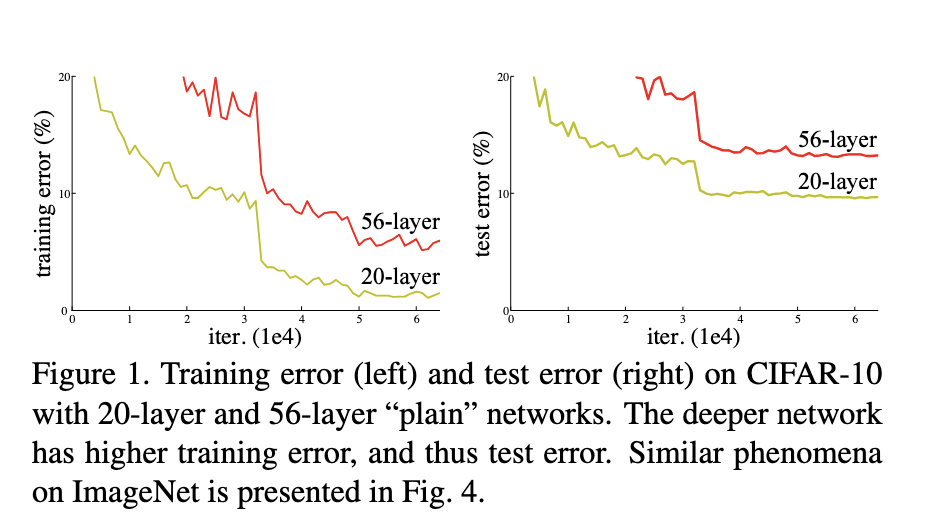
\includegraphics[width=0.5\textwidth]{./images/Screenshot 2025-05-20 at 0.22.01.png}
	\end{figure}
\end{frame}

\begin{frame}
	\frametitle{Introduction}

	\textbf{It should be possible for deeper networks to perform at least as well as their shallower counterparts.}
	
	\begin{itemize}
		\item The degradation (of training accuracy) indicates that not all systems are similarly easy to optimize.
		\item There exists a solution by construction to the deeper model.
		\item The existence of this constructed solution indicates that a deeper model should produce no higher training error than its shallower counterpart.
		\item This paper describes how residual learning and shortcut connections work together to solve the degradation problem.
	\end{itemize}
\end{frame}

\begin{frame}
	\frametitle{Related Work}

	\textbf{These two ideas (residual representations, shortcut connections) already used in the other works}
	\begin{itemize}
		\item Residual Representations.
		\begin{itemize}
			\item Classic computer vision techniques, such as VLAD and Fisher Vectors, encode “residuals” (i.e., differences from some representative value or dictionary entry) rather than raw features.
		\end{itemize}
		\item Shortcut Connections.
		\begin{itemize}
			\item Early MLP variants that included linear connections from input to output use the same idea.
			\item The novelty of ResNet lies in using only parameter-free shortcuts (pure identity mapping) and always learning residual functions.
		\end{itemize}
	\end{itemize}
\end{frame}

\begin{frame}
	\frametitle{Related Work}

	\textbf{The novelty of ResNet lies in using these method in deep networks to optimize training.}
	\begin{itemize}
		\item Previous methods have not demonstrated successful training of very deep networks (100+ layers) without optimization issues, especially using only identity shortcuts and residual mappings.
		\item The authors assert their simple, general approach—stacking residual blocks with identity shortcuts—addresses optimization challenges for deep models and outperforms prior strategies.
	\end{itemize}
\end{frame}

\begin{frame}
	\frametitle{Deep Residual Learning}

	\textbf{3.1. Residual Learning}

	\begin{itemize}
		\item We address the degradation problem by introducing a Deep residual learning framework.
		\item Instead of making layers directly fit a desired mapping \( H(x) \), we let them fit a residual mapping:
	\end{itemize}

	\begin{exampleblock}{Residual Mapping}
		Given \( H(x) \), let  
		\[
		F(x) := H(x) - x \quad \Rightarrow \quad H(x) = F(x) + x
		\]
	\end{exampleblock}

	\begin{itemize}
		\item We hypothesize it's easier to optimize \( F(x) \) than \( H(x) \) directly.
	\end{itemize}
\end{frame}

\begin{frame}
	\frametitle{Deep Residual Learning}

	\textbf{3.1. Residual Learning}

	\begin{block}{Identity Mapping Case}
		If the identity mapping is optimal, pushing \( F(x) \rightarrow 0 \) is easier than approximating \( H(x) = x \) via nonlinear layers.
	\end{block}

	\begin{itemize}
		\item This is implemented with shortcut connections, which skip one or more layers and perform identity mapping.
	\end{itemize}

	\begin{alertblock}{No Overhead, Easy Integration}
		Shortcut connections add no extra parameters or computation.  
		Training can proceed end-to-end using SGD and backpropagation.  
		Easily implementable with standard libraries (e.g., Caffe).
	\end{alertblock}
\end{frame}

\begin{frame}
    \frametitle{Deep Residual Learning}

    \textbf{3.2. Identity Mapping by Shortcuts}
    \begin{equation}
        y = F(x, \{W_i\}) + x
    \end{equation}
    \vspace{-2mm}
    \begin{itemize}
        \item $x$: Input vector
        \item $y$: Output vector
        \item $F(x, \{W_i\})$: Residual function (e.g., two-layer MLP or CNN)
    \end{itemize}
    \vspace{2mm}
    \textbf{Example:}
    \[
        F = W_2 \sigma(W_1 x)
    \]
    where $\sigma$ is ReLU and biases are omitted.

	\begin{figure}
		\centering
		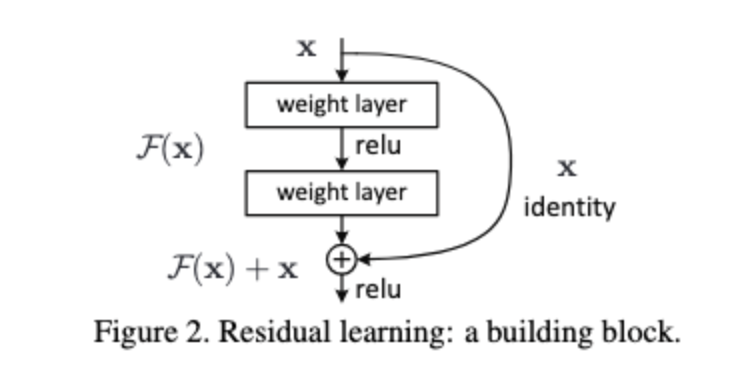
\includegraphics[width=0.5\textwidth]{./images/Screenshot 2025-05-20 at 0.19.36.png}
	\end{figure}
\end{frame}

\begin{frame}
    \frametitle{Deep Residual Learning}

    \textbf{3.2. Identity Mapping by Shortcuts}

    \textbf{When Dimensions Differ:}
    \begin{equation}
        y = F(x, \{W_i\}) + W_s x
    \end{equation}

    \begin{itemize}
        \item $W_s$: Projection matrix (e.g., $1 \times 1$ convolution).
        \item Used to match dimensions of $x$ and $F(x)$.
    \end{itemize}

    \textbf{Note:} Identity mapping ($W_s = I$) is sufficient in most cases.

	\begin{figure}
		\centering
		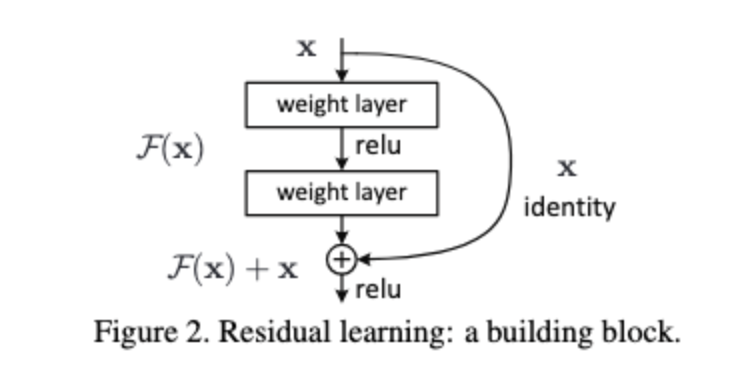
\includegraphics[width=0.5\textwidth]{./images/Screenshot 2025-05-20 at 0.19.36.png}
	\end{figure}
\end{frame}

\begin{frame}
	\frametitle{Network Architectures}
	
	\begin{columns}
		\begin{column}{0.5\textwidth}
			\begin{itemize}
				\item Based on the plain network, we insert shortcut connections which turn the network into its counterpart residual version.
				\item When the dimensions increase: 
				\begin{itemize}
					\item[(A)] The shortcut still performs identity mapping, with extra zero entries padded for increasing dimensions.
					\item[(B)] The projection shortcut in Eqn.(2) is used to match dimensions (done by 1×1 convolutions).
				\end{itemize}
			\end{itemize}
		\end{column}
		\begin{column}{0.6\textwidth}
			\centering
			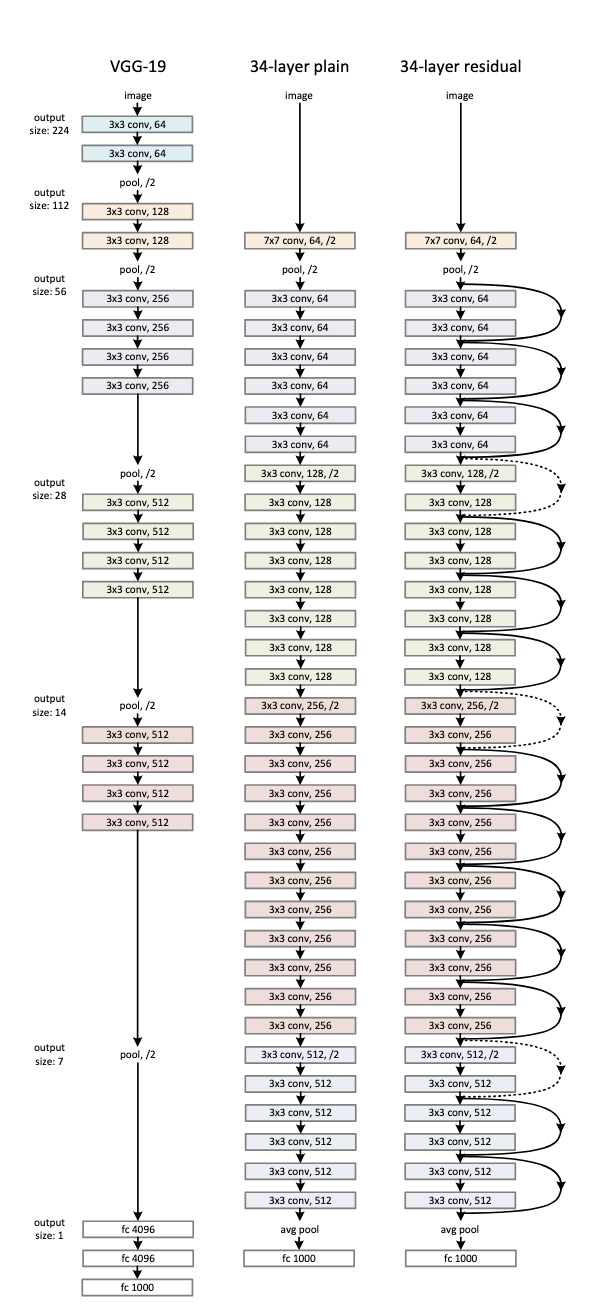
\includegraphics[width=0.5\linewidth]{./images/Screenshot 2025-05-20 at 0.25.50.png} % 画像ファイル名を指定(拡張子不要)
		\end{column}
	\end{columns}
\end{frame}

\begin{frame}
	\frametitle{Implementation}
	
	\begin{itemize}
		\item 224 × 224 cropping
		\item color augumentation and horizontal flipping
		\item adopt batch normalization right after each convolution and before activation
		\item use He initialization to initialize weights
		\item the models are trained for up to 60 × 104 iterations
		\item use a weight decay of 0.0001 and a momentum of 0.9 for SGD
		\item do not use dropout (\textit{Batch Normalization allows us to
use much higher learning rates and be less careful about initialization, and in some cases eliminates the need for Dropout})
	\end{itemize}
\end{frame}

\begin{frame}
	\frametitle{Experiments}

	\textbf{4.1. ImageNet Classification}

	\begin{itemize}
		\item use datasets that consists of 1000 classes
		\item 1.28 million training images
		\item 50k validation images
		\item 100k test images
		\item evaluate both top-1 and top-5 error rates
	\end{itemize}
\end{frame}

\begin{frame}
	\frametitle{Experiments}

	\textbf{We argue that this optimization difficulty is unlikely to be caused by vanishing gradients.}

	\begin{figure}
		\centering
		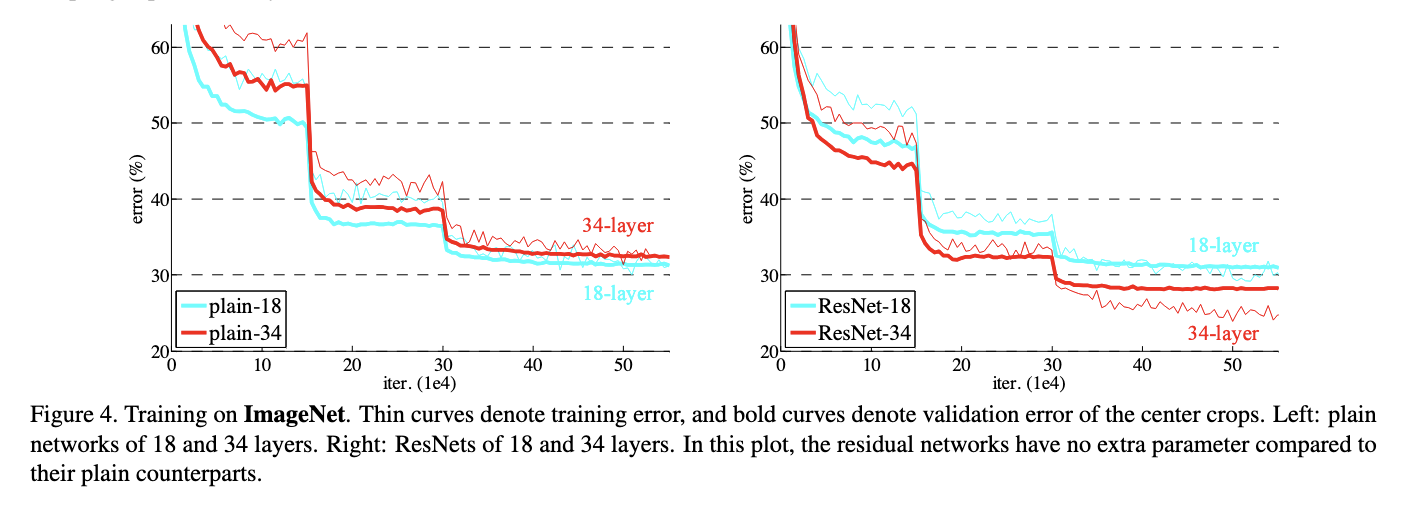
\includegraphics[width=0.8\textwidth]{./images/Screenshot 2025-05-20 at 0.33.26.png}
	\end{figure}

	\begin{figure}
		\centering
		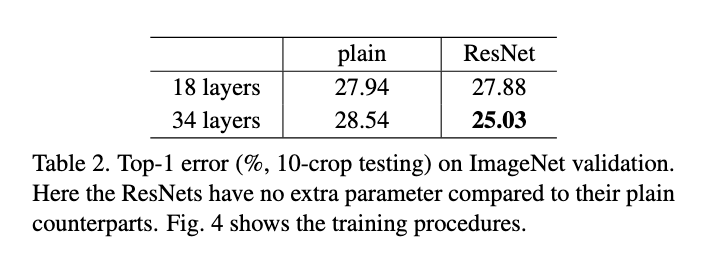
\includegraphics[width=0.7\textwidth]{./images/Screenshot 2025-05-20 at 0.33.49.png}
	\end{figure}
\end{frame}

\begin{frame}
	\frametitle{Experiments}

	\textbf{the small differences among A/B/C indicate that projection shortcuts are not essential for addressing the degradation problem.}

	\begin{figure}
		\centering
		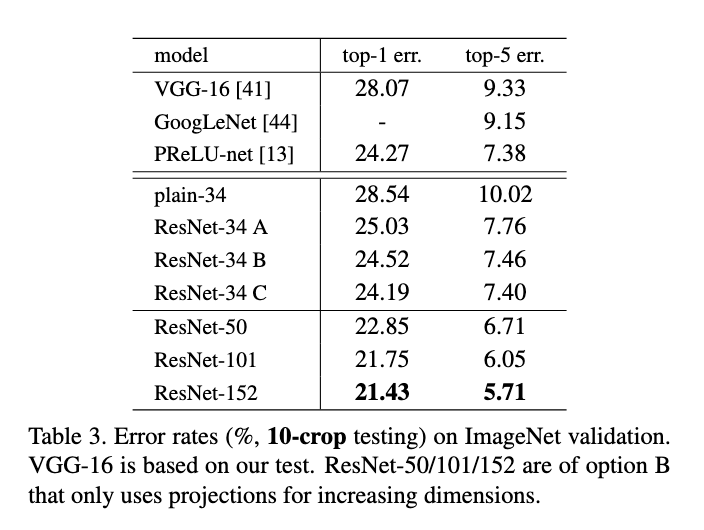
\includegraphics[width=0.8\textwidth]{./images/Screenshot 2025-05-20 at 0.34.01.png}
	\end{figure}
\end{frame}

\begin{frame}
	\frametitle{Experiments}

	\textbf{Bottleneck Architecture}

	\begin{itemize}
		\item we modify the building block as a bottleneck design
		\item For each residual function F, we use a stack of 3 layers instead of 2
		\item The three layers are 1×1, 3×3, and 1×1 convolutions, where the 1×1 layers are responsible for reducing and then increasing (restoring) dimensions, leaving the 3×3 layer a bottleneck with smaller input/output dimensions.
		\item The parameter-free identity shortcuts are particularly important for the bottleneck architectures.
	\end{itemize}

	\begin{figure}
		\centering
		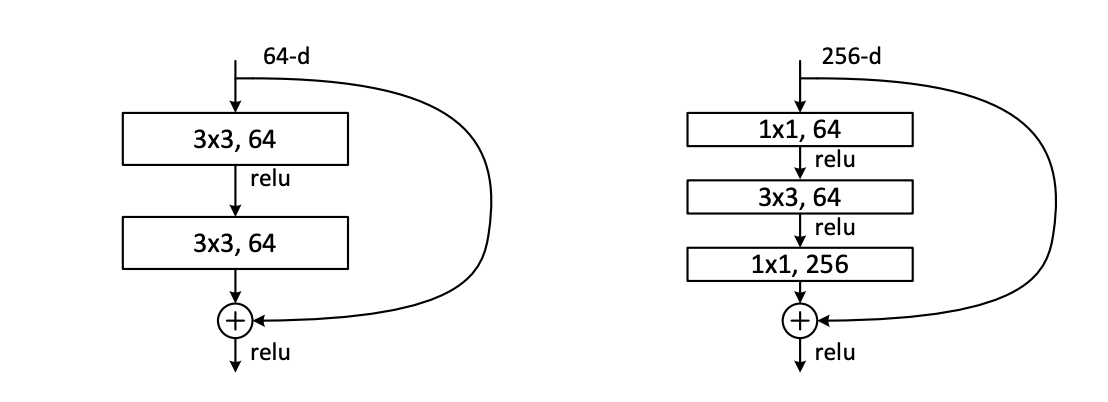
\includegraphics[width=0.6\textwidth]{./images/Screenshot 2025-05-20 at 12.17.56.png}
	\end{figure}
\end{frame}

\begin{frame}
	\frametitle{Experiments}

	\textbf{ResNet showed significant improvements even with deep network.}

	\begin{figure}
		\centering
		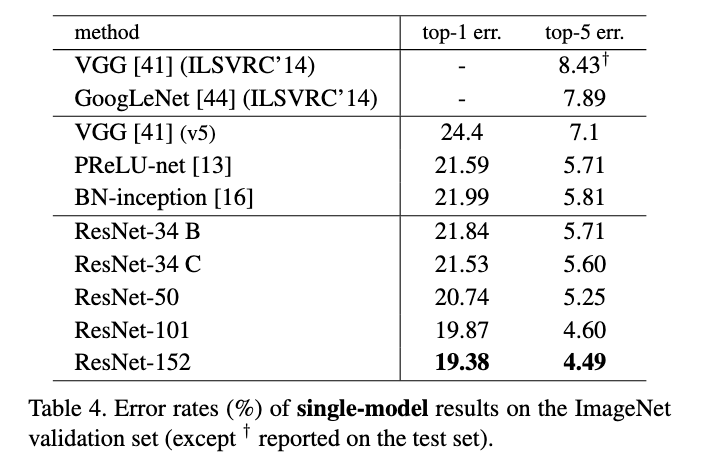
\includegraphics[width=0.8\textwidth]{./images/Screenshot 2025-05-20 at 0.34.11.png}
	\end{figure}
\end{frame}

\begin{frame}
	\frametitle{Experiments}

	\begin{figure}
		\centering
		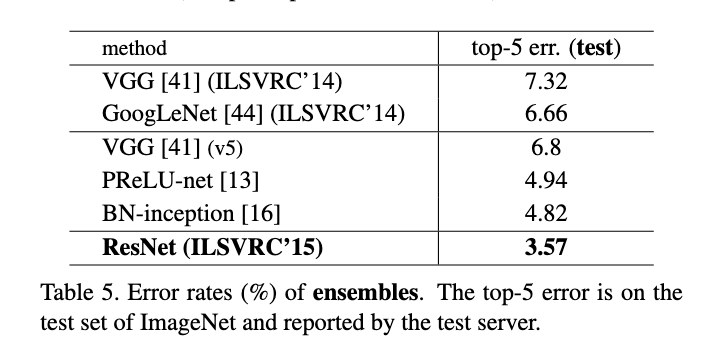
\includegraphics[width=0.8\textwidth]{./images/Screenshot 2025-05-20 at 0.34.30.png}
	\end{figure}
\end{frame}

\begin{frame}
	\frametitle{Experiments}

	\textbf{4.2. CIFAR-10 and Analysis}

	\begin{itemize}
		\item CIFAR-10 dataset, which consists of 50k training images
		\item 10k testing images
		\item 10 classes
		\item Our focus is on the behaviors of extremely deep networks, but not on pushing the state-of-the-art results, so we intentionally use simple architectures
		\item residual models have exactly the same depth, width, and number of parameters as the plain counterparts
	\end{itemize}
\end{frame}

\begin{frame}
	\frametitle{Experiments}

	\textbf{It has fewer parameters than other deep and thin networks such as FitNet and Highway. }

	\begin{figure}
		\centering
		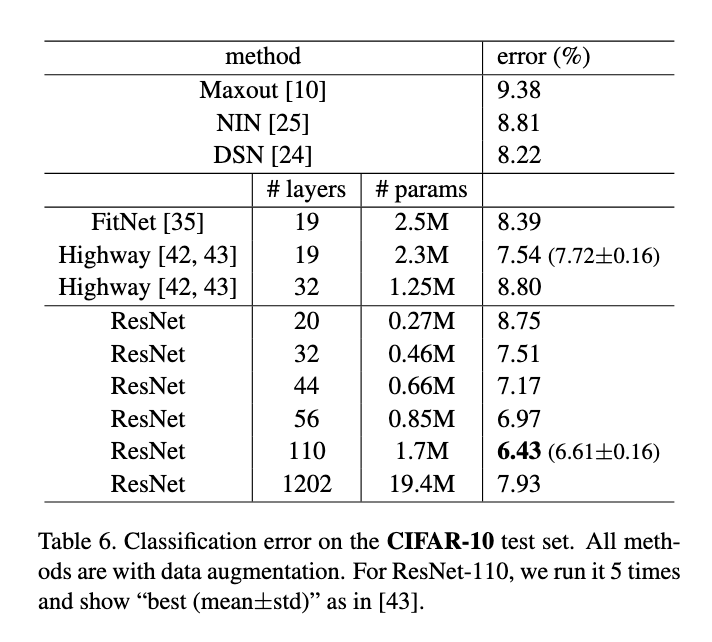
\includegraphics[width=0.65\textwidth]{./images/Screenshot 2025-05-20 at 0.40.29.png}
	\end{figure}
\end{frame}


\begin{frame}
	\frametitle{Experiments}

	\begin{figure}
		\centering
		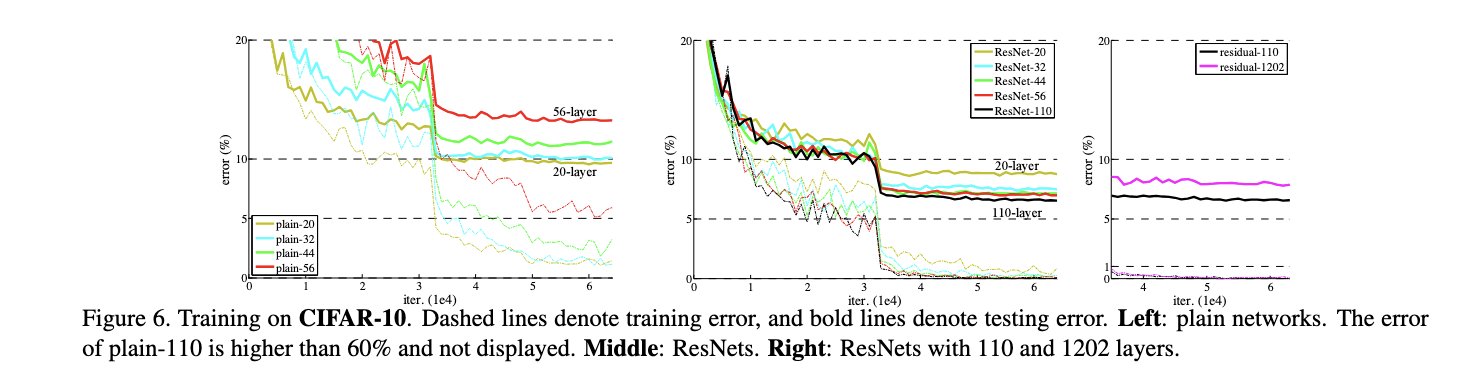
\includegraphics[width=\textwidth]{./images/Screenshot 2025-05-20 at 0.41.53.png}
	\end{figure}
\end{frame}

\begin{frame}
	\frametitle{Experiments}

	\textbf{ResNets have generally smaller responses than their plain counterparts}\\
	\textbf{The deeper ResNet has smaller magnitudes of responses.}

	\begin{figure}
		\centering
		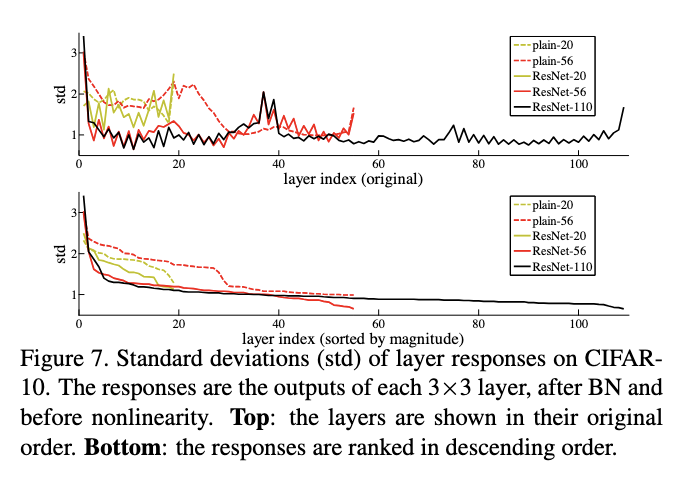
\includegraphics[width=0.8\textwidth]{./images/Screenshot 2025-05-20 at 0.42.53.png}
	\end{figure}
\end{frame}

\begin{frame}
	\frametitle{Experiments}

	\textbf{4.3. Object Detection on PASCAL and MS COCO} 

	\begin{figure}
		\centering
		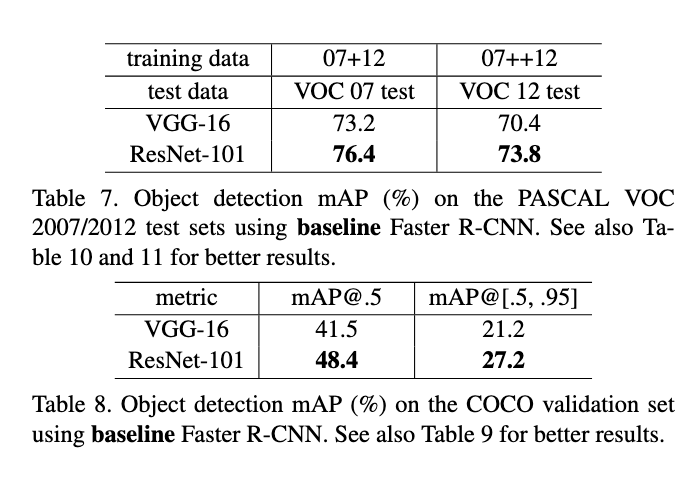
\includegraphics[width=0.7\textwidth]{./images/Screenshot 2025-05-20 at 0.44.13.png}
	\end{figure}
\end{frame}

\begin{frame}
	\frametitle{Appendix}

	\begin{figure}
		\centering
		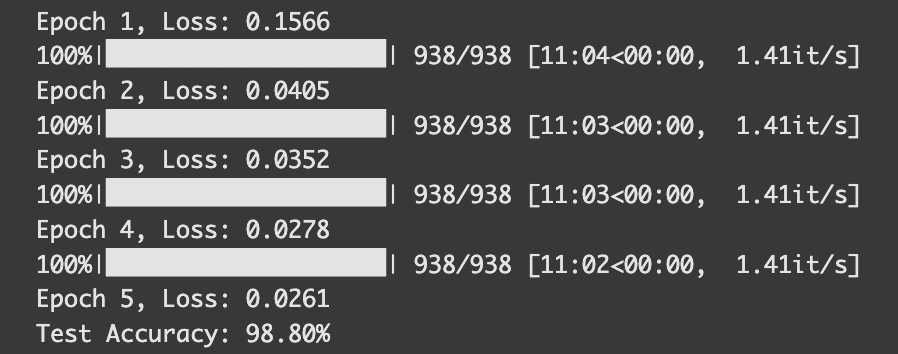
\includegraphics[width=\textwidth]{./images/Screenshot 2025-05-20 at 9.51.40.png}
	\end{figure}

	Ref: \url{https://zenn.dev/takeguchi/articles/f6b4530d57177e}
\end{frame}
\end{document} 
